\apendice{Documentación técnica de programación}

%%INTRODUCCION
\section{Introducción}
En este anexo se describe la documentación técnica de programación para este proyecto. Incluye los primeros pasos que son la instalación del proyecto, la estructura de la aplicación o finalmente como compilarlo, desplegarlo o los diferentes tipos de configuraciones realizados. La idea es poder facilitar a los futuros desarrolladores una guía con la que poder comenzar, en el caso de que quisieran continuar con el trabajo.

%% eSTRUCTURA DE DIRECTORIOS
\section{Estructura de directorios}
El repositorio se encuentra alojado en \href{https://github.com/scc0034/flutter_serpiente}{Github}. La estructura de ficheros más relevantes que tiene el proyecto es la siguiente:

\begin{itemize}
\item \textbf{./}
Directorio raíz del que cuelgan todas los demás ficheros. Este contiene uno de los archivos más importantes, que es es \emph{pubspec.yalm}. Este archivos se usa para hacer las importaciones de lós paquetes con las funcionalidades que queramos dar a nuestra aplicación.

\begin{itemize}
	\item \textbf{build}: Este directorio contiene todo lo relativo a las compilaciones, es decir, tanto como para hacer las pruebas en local de la aplicación, o crear los \emph{releases} que creamos oportunos. Además contiene todo lo relativo a las conexiones con Android Studio y Firebase, ya que necesita hacer las llamadas a este para lanzar los emuladores con la máquina virtual correspondiente. Dentro de esta estructura algunos de los ficheros más importantes son:
	\begin{itemize}
		\item \textbf{key.properties}: propiedades de la key, ya que esta nos permite desplegar la aplicación en la \emph{Play Store}. Es algo que no se tiene que perder ni modificar, ya que es de sumo valor. 
		\item \textbf{app/google-services.json}: fichero que descargamos desde Firebase, para que la aplicación tenga las conexiones con este \emph{Cloud service}, es decir, contienen las claves de conexión. En el caso de que tengamos que lanzar la app con otro de servicio de Firebase, podemos hacerlo cambiando este fichero.
		\imagen{techprog/google-services.jpg}{Google services}
		\item \textbf{app/build.gradle}: Fichero que contiene lo necesario para hacer las compilaciones, ya que como vemos tiene el SDK mínimo y máximo con el que trabaja (limitando el número de dispositivos que son compatibles). El número de versión para cuando sea subido a la \emph{Play Store}, es algo que se debe revisar siempre, ya que si no vamos a tener problemas de versionado. Además de los parámetros usados en la clave como podemos ver en la siguiente imagen.
		\imagen{techprog/app_build_gradle.jpg}{app/build.gradle}
		\item \textbf{app/key/keysnake.jks}: clave cifrada generada mediante el comando \ref{fig:commandkey}, esta no se puede perder, ya que sin ella es imposible desplegar la aplicación en la \emph{Play Store}. Es conveniente hacer alguna copia de seguridad en local.
		
		\begin{figure}[H]
			\centering
			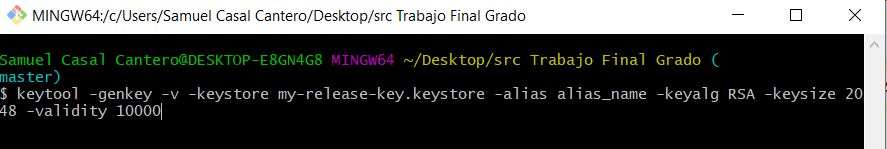
\includegraphics[width=1.0\textwidth]{/techprog/keysnakecommand}
			\caption{Comando generar clave keyStore}
			\label{fig:commandkey}
		\end{figure}	 
	\end{itemize}
	\item \textbf{assets}: directorio que contiene los archivos de imágenes y audio de la aplicación. 
	\item \textbf{data/menu-opt.json}: fichero \emph{json} con la estructura del menú \emph{drawer}, con los nombres de ruta, nombre de icono y nombre de la página. 
	\item \textbf{docs/latex}: memoria y anexos del trabajo final de grado.
	\item \textbf{lib}: contiene los ficheros que se compilan para crear la aplicación. La estructura interna de directorios es la siguiente:
	\begin{itemize}
		\item \textbf{main.dart}: fichero principal del que cuelga toda la aplicación.
		\item \textbf{models}: contiene los modelos para crear las instancias de los objetos de la base de datos.
		\item \textbf{pages}: cada una de las interfaces o páginas de la aplicación.
		\item \textbf{providers}: proveedores de algunos servicios internos.
		\item \textbf{routes}: rutas de la aplicación.
		\item \textbf{services}: instancias a los servicios externos de la aplicación.
		\item \textbf{utils}: utilidades.
		\item \textbf{widgets}: elementos gráficos reutilizables.
		 
	\end{itemize}
\end{itemize}
\end{itemize}

%% MANUAL DEL PROGRAMADOR
\section{Manual del programador}
Este manual del programador tiene como objetivo ayudar a personas que en un futuro estén interesadas en la continuación del proyecto, o simplemente que tengan ganas de aprender como se ha realizado. Para ello debemos de realizar las instalaciones de las siguientes herramientas:

\begin{itemize}
	\tightlist
	\item Flutter.
	\item Android Studio.
	\item Visual Studio Code.
	\item Git.
	\item Firebase Console.
	\item Play Store Console.
\end{itemize}

\subsection{Flutter:}
Es un SDK de código abierto creado por Google. Ofrece la versatilidad de crear aplicaciones móviles tanto como para \emph{iOS} y \emph{Android}, pero también para el entorno web. Internamente el lenguaje de programación es Dart.js, un \emph{framework}, que también es \emph{Open Source} desarrollado por Google, ya que pretende mejorar algunas de las carencias que tiene \emph{javascript}.

Para la instalación de Flutter debemos de ir a su \href{https://flutter.dev/docs/get-started/install}{web oficial} y descargarlo, dependiendo del sistema operativo que tengamos usaremos una versión u otra. (v.17.5 \emph{stable}).

Al descomprimir el fichero nos daremos cuenta de que tenemos un directorio (no ejecutable), por lo que debemos de dejar este en un lugar en concreto para después añadirlo a las variables de usuario. En mi caso lo dejé en la siguiente ruta de mi ordenador personal C:$\backslash$src$\backslash$flutter.

Una vez realizado el paso anterior debemos de actualizar las variables de usuario, apuntando al directorio bin de la ruta anterior, como vemos en la siguiente imagen:

\imagen{techprog/variablesEntorno.jpg}{Variables entorno}

Por defecto la rama de Flutter es la \emph{stable}, de las ramas disponibles: \emph{stable, beta, dev, master}. Pero si en el caso de necesitar la misma versión de Flutter, el comando necesario es:

\imagen{techprog/version}{Comando version Flutter}


\subsection{Android Studio:}
Es el IDE oficial de Google, que remplaza a Eclipse, basado en \emph{IntelliJ IDEA}, publicado de manera gratuita con Licencia Apache 2.0.

En nuestro caso, no programaremos en este IDE, ya que es complicado trabajar con Flutter directamente, solo lo vamos a utilizar para la creación de las máquinas virtuales para emular el sistema operativo Android. Por lo que descargamos de la \href{https://developer.android.com/studio}{web oficial Android Studio} e instalamos, en mi caso utilicé la versión 3.6.

Una vez instalado, creamos las máquinas virtuales. Para ello se va a la barra de herramientas Tools>AVD manager y se crean las que sean necesarias,. En mi caso tengo dos, ambas con Andorid R, que es la versión 10 de sistema operativo, ya que es la última estable que nos ofrece el IDE.
\imagen{techprog/vm.jpg}{Máquinas virtuales}

\subsection{Visual Studio Code:}
Es el editor de código creado por Microsoft, permite mucha versatilidad y es eficiente para la edición del código en flutter. Es de código abierto bajo la licencia MIT.

Lo podemos descargar de la \href{https://code.visualstudio.com/}{web VS Code}, en mi caso uso la versión 1.47.

Una vez lo tengamos instalado, procedemos a instalar los siguientes \emph{Snippets} que nos ayudan a la creación del código, ya que son como los atajos de teclado. En cada uno de los enlaces, podemos ver una descripción de cada una de estas herramientas:

\begin{itemize}
	\tightlist
	\item \href{https://marketplace.visualstudio.com/items?itemName=Nash.awesome-flutter-snippets}{Awesome Flutter Snippets}. Apache 2.0.
	\item \href{https://marketplace.visualstudio.com/items?itemName=CoenraadS.bracket-pair-colorizer-2}{Bracket Pair Colorizer 2}. MIT License.
	\item \href{https://marketplace.visualstudio.com/items?itemName=Dart-Code.dart-code}{Dart}. MIT License.
	\item \href{https://marketplace.visualstudio.com/items?itemName=Dart-Code.flutter}{Flutter}. MIT License.
\end{itemize}

\subsection{Git:}
Es un software para el control de las versiones, que nos permite trabajar mediante comandos desde \emph{Git Bash}, la licencia es GNU-GPL v2.  La última versión estable con la que he trabajado es 2.27 y la podemos encontrar \href{https://git-scm.com/}{web oficial}.

\subsection{Firebase Console:}
La consola de \href{https://console.firebase.google.com/?hl=es}{Firebase} es la que nos permite el control de todas las características de \emph{Cloud Services}, desde la autentificación de los usuarios, base de datos o AdMob services, entre otras muchas.

Al estar registrado con mi cuenta personal, tendría que dar permisos de administrador en el caso de que fuera necesario, para ello pueden mandarme un correo a \href{mailto:casalyepa@gmail.com}{casalyepa@gmail.com}

\imagen{techprog/firebase.jpg}{Firebase console}

\subsection{Play Store Console:}
La consola de \href{https://play.google.com/apps}{Play Store} es la herramienta web que nos permite hacer el despligue de la aplicación, hacer las pruebas alfa y beta, o para subirla y que todo el mundo se la pueda descargar.

La revisión de cada una de las nuevas versiones puede tardar en ser validada, por lo que se debe tener paciencia.

Al igual que con Firebase, tendría que dar permisos en el caso de que sea necesario hacer nuevos despliegues de la app, correo a \href{mailto:casalyepa@gmail.com}{casalyepa@gmail.com}

\imagen{techprog/playstore.jpg}{Play Store console}

%% 	COMPILACIÓN DEL PROYECTO INSTALACIÓN Y EJECUCION
\section{Compilación, instalación y ejecución del proyecto}
En este apartado se muestran los pasos necesarios para hacer una copia del proyecto en Github y poder trabajar en local desplegando la aplicación en los emuladores.

\subsection{Clonación del proyecto:}

\begin{enumerate}
	\item Nos colocamos en el directorio donde queramos tener el proyecto y abrimos \emph{git bash} mediante el botón derecho:\imagen{techprog/clonar.png}{Abrir git bash}
	\item Procedemos a clonar el proyecto con el comando : 
	\texttt{git clone \\https://github.com/scc0034/flutter\_serpiente.git}~\ref{fig:git-clone}
\end{enumerate}

\begin{figure}[H]
	\centering
	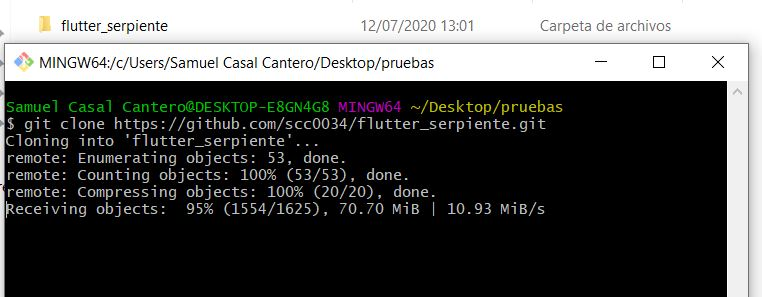
\includegraphics[width=1\textwidth]{techprog/gitclone.jpg}
	\caption{Comando para clonar el repositorio.}\label{fig:git-clone}
\end{figure}

\subsection{Instalación de los paquetes:}
Una vez esté el proyecto clonado, se debe ejecutar el comando \texttt{flutter upgrade}, para traer todos los paquetes, ya que si no en las importaciones de cada uno de los ficheros van a aparecer como erróneas.

\begin{figure}[H]
	\centering
	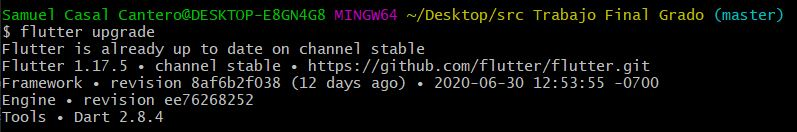
\includegraphics[width=1\textwidth]{techprog/flutterupgrade.jpg}
	\caption{Actualización de paquetes}\label{fig:upgrade}
\end{figure}

Una vez realizado debemos reiniciar Visual Studio Code.

\subsection{Ejecución del proyecto:}
Se puede hacer de tres maneras diferentes:

\begin{enumerate}
	\item Descargar la última versión subida a la \href{https://play.google.com/store/apps/details?id=com.ubu.flutter_snake}{Play Store}, esto solo es válido para el despliegue de la aplicación, no para desarrollo. Por los tiempos de despliegue.

	\item Desde la consola de git, \texttt{flutter devices}, para ver que dispositivos tenemos disponibles, en el caso de que dentro de la lista no se muestre nada, se debe de ir a Andorid Studio y arrancar una de las máquinas virtuales~\ref{fig:run} .
	Si la lista presenta dispositivos, ejecutamos el siguiente comando \texttt{flutter run -d emulator-id}, siendo el id, el número de la máquina virtual que muestra el comando anterior.
	
	\item Desde Visual Studio Code (se debe tener las herramientas de visual studio), se da al \texttt{F5}, se mostrará una lista con los dispositivos encontrados en el sistema. En el caso de que se disponga de un móvil físico conectado, aparecerá también en la lista anterior. Finalmente arrancará la aplicación en el terminal seleccionado.\ref{fig:run}.
\end{enumerate} 	

\begin{figure}[H]
	\centering
	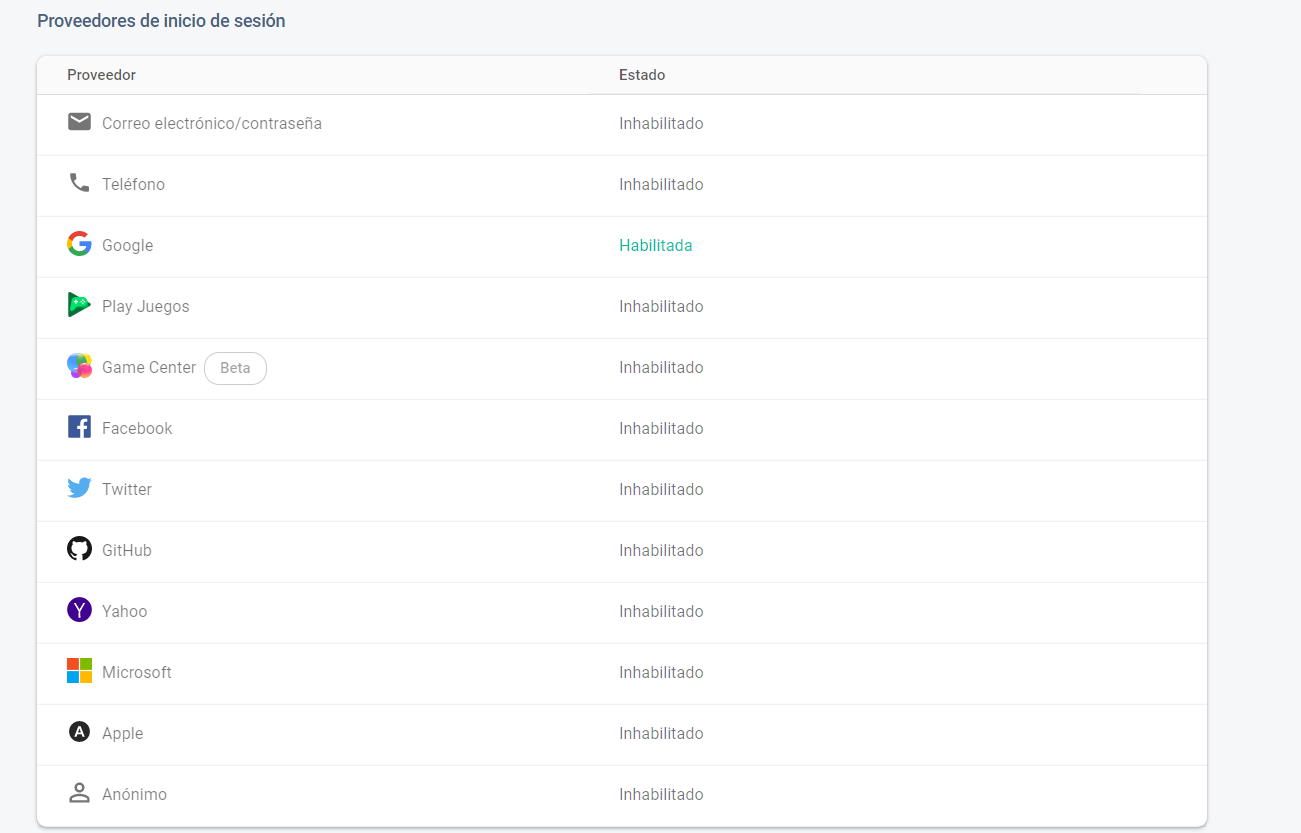
\includegraphics[width=1\textwidth]{techprog/inicio.jpg}
	\caption{Máquina virtual}\label{fig:run}
\end{figure}

\subsection{Generar los apks}
Hay dos opciones para generar los ficheros, dependiendo del destino de cada uno de ellos, es decir, las opciones que se encuentran son la siguientes:
\begin{enumerate}
	\item \textbf{Para la tienda:} Generar el \emph{bundle}~\cite{wiki:bundle} para hacer el despliegue en \emph{Play Store}, para ello el comando que se ha de escribir en la consola es: \texttt{flutter build appbundle}. Se genera un archivo \emph{.aab}, de tal forma que dependiendo de que dispositivo descargue la app, desde la tienda, se baje unos archivos u otros, con el fin de que la aplicación pese menos.  Antes de generar el nuevo \emph{bundle}, se debe mirar que versión de la app tiene la tienda, para cambiar la versión de la aplicación en local a una mayor, de tal forma que al subirla no se den problemas de incompatibilidad. En la salida por pantalla del comando nos dice en que ruta se encuentran los ficheros generados.
	\item \textbf{Apks:} Generar las apks para cada uno de los sistemas: \texttt{flutter build apk --releases}. En la ejecución del comando se muestra la ruta donde se encuentran los ficheros generados.
\end{enumerate} 

%% PRUEBAS DEL SISTEMA
\section{Pruebas del sistema}
Para validar el correcto funcionamiento del producto, se han realizado diferentes tipos de pruebas: unitarias, de integración y de sistema. Hay que destacar que Flutter tiene herramientas para la automatización de test (\emph{Appian} es una de ellas), pero debido a lo ajustado que está el proyecto, no se han realizado mediante estas, ya que no se pueden grabar los test como con \emph{Selenium}, por poner un ejemplo similar. 

Es decir, se puede considerar como línea de trabajo futura, con metodologías de programación dirigida por los test, como es el caso de \empt{Test-Driven Development}.

\subsection{Pruebas unitarias:}
Se han realizado de forma simple o \emph{hardcodeando prints} en el propio código y mostrándolos por el terminal en tiempo de ejecución. En el caso de continuar con el desarrollo sería imprescindible trabajar con test automáticos. Han validado pequeños módulos o fragmentos de código, con el fin de garantizar de que estas pequeñas unidades funcionen. Uno de los ejemplos es~\ref{fig:impacto}:

\begin{figure}[H]
	\centering
	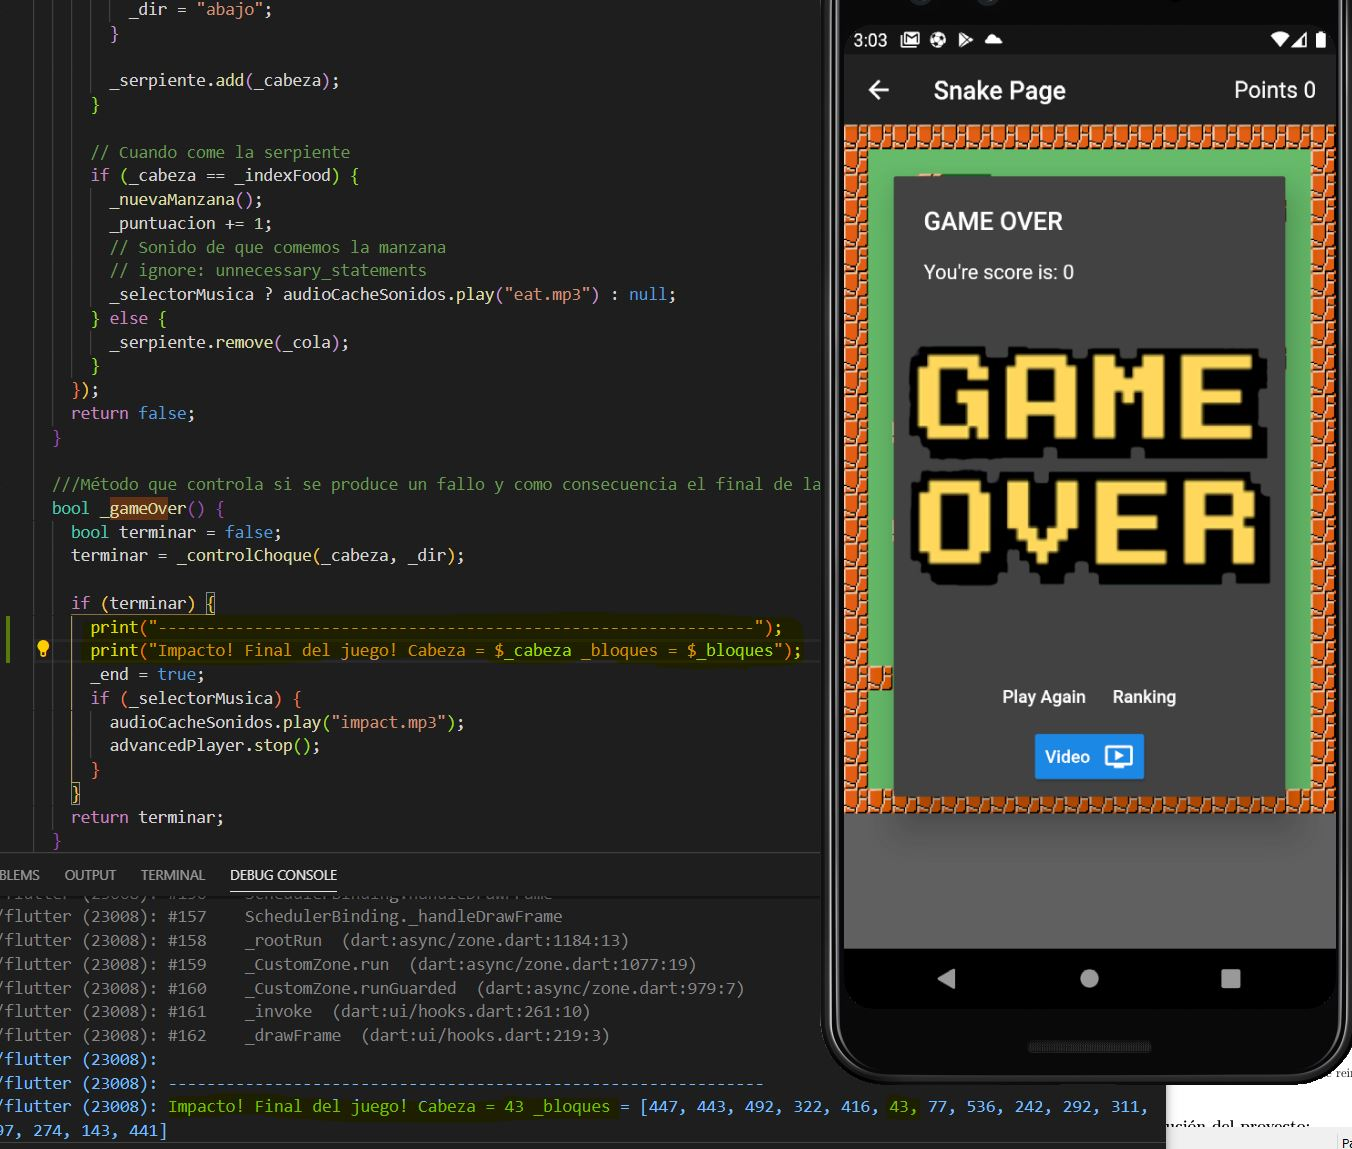
\includegraphics[width=1\textwidth]{techprog/impacto.jpg}
	\caption{Máquina virtual}\label{fig:impacto}
\end{figure}

\subsubsection{Pruebas de caja negra:}
En ocasiones se han realizado casos de prueba de caja negra para algunas líneas de código~\ref{fig:codigocontrolchoque}. Para realizar las pruebas es necesario construir las tablas con clases de equivalencia válidas y no válidas~\ref{table:casosNegros}. Después la tabla de los diferentes casos de prueba con los resultados obtenidos~\ref{table:derivacion}.

\begin{figure}[H]
	\centering
	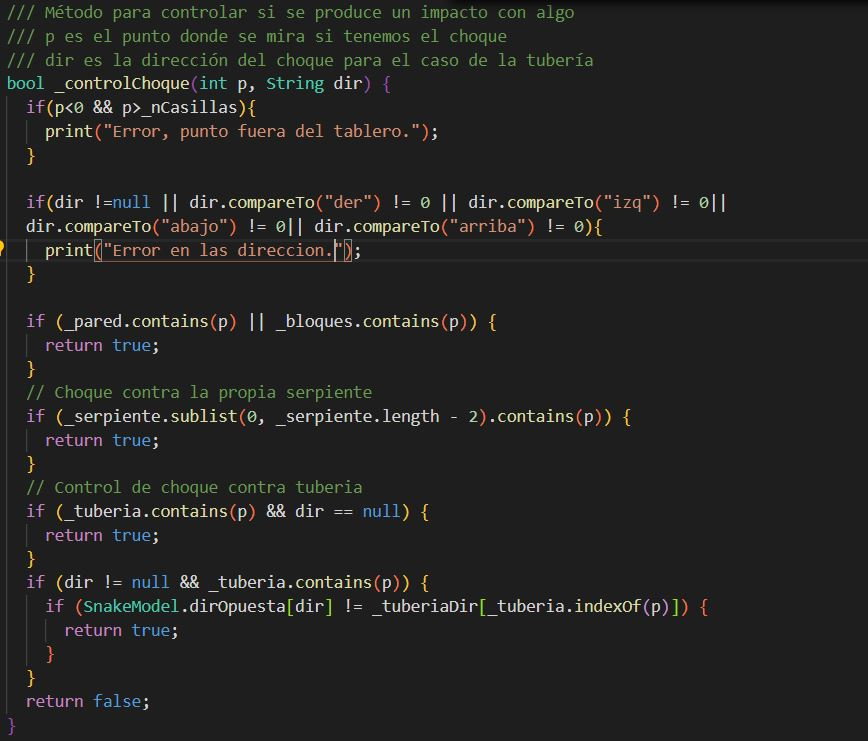
\includegraphics[width=1\textwidth]{techprog/codigocontrolchoque.jpg}
	\caption{Código para las pruebas de caja negra}\label{fig:codigocontrolchoque}
\end{figure}

Dando como resultado las dos tablas siguientes:

La primera de las tablas define las clases de equivalencia que son válidas y las que no.
\rowcolors {2}{gray!35}{}
\begin{table}[H]
	\begin{center}
		\begin{tabular}{ccc}
			\hline
			Condición entrada		& Clase válida		& Clase no válida \\ \hline
			p dentro del tablero	&1. p>0 AND p<n celdas		&2. p<0 AND p>n celdas\\
			dir debe ser válida		&3. null,der,izq,abajo,arriba		&4. dir no válida\\
		\end{tabular}
		\caption{Clases de equivalencia}
		\label{table:casosNegros}
	\end{center}
\end{table}

La segunda tabla es una comprobación de lo que sucede para cada una de las clases de equivalencia. Dependiendo de si se produce choque con alguno de los elementos se devuelve true, en caso contrario false.
\rowcolors {2}{gray!35}{}
\begin{table}[H]
	\begin{center}
		\begin{tabular}{ccc}
			\hline
			Entrada		& Clase cubierta		& Resultado \\ \hline
			p =	10		&1(clase válida)		&return true/false\\
			p =	-2		&2						&Mensaje error\\
			p =	600		&2						&Mensaje error\\
			dir = null  &3(clase válida)		&return true/false\\
			dir = der   &3(clase válida)		&return true/false\\
			dir = izq   &3(clase válida)		&return true/false\\
			dir = abajo &3(clase válida)		&return true/false\\
			dir = arriba&3(clase válida)		&return true/false\\
			dir = diag	&4						&Mensaje error\\
		\end{tabular}
		\caption{Derivación en casos de prueba de caja negra}
		\label{table:derivacion}
	\end{center}
\end{table}

Tras realizar los casos de caja negra, como es el caso anterior, me he dado cuenta de que es imprescindible la automatización de los test. Ya que nos ahorra gran cantidad de tiempo, y en el momento que la aplicación falle, veremos si se produce el error.

\subsection{Pruebas de integración y sistema:}
Confirmar que el conjunto de módulos anteriormente validados, funcionen todos de manera interrelacionada unos con otros. Para ello lo que se ha hecho es un testeo de funcionamiento en el terminal físico, lo que conlleva un \emph{testing} simultáneo de la interfaz. 

Muchos de los errores son más fáciles de encontrar así, porque en la máquina virtual no funciona de la misma manera, ya que el rendimiento no es el mismo, o las simulaciones son parciales. Uno de los ejemplos que fue necesario hacer \emph{in situ}, fue el juego online, a la hora de tener que validar que se producían las conexiones entre los terminales.

En estas pruebas de interfaz, se encontraron algunos campos que no eran visibles de manera correcta o que su usabilidad era reducida. Lo que supuso la realización de la mejora correspondiente.

\subsection{Pruebas de despliegue de la aplicación}
Este tipo de pruebas es algo muy complejo de controlar, ya que, hasta desplegamos la aplicación en la tienda, algunos de los errores permanecen enmascarados, durante el proceso de implementación. Esto es debido a trabajar con máquinas virtuales, capadas en algunos aspectos o simplemente que es un compilado de la aplicación instalada, sin tener que pasar por la tienda. O simplemente que no es el entorno real de usuario.

Por lo que para ello sería muy recomendable hacer unas pruebas de beta cerrada, ya que la plataforma de \emph{Play Store Console}, tenemos opciones para ello.